\chapter{Ionización del medio y simulaciones Monte Carlo}
\textcolor{red}{Esta sección va a tener que ser totalmente refactorizada:
\begin{itemize}
    \item Podría empezar con una introducción \textit{teórica} del fenómeno físico, poder explicarlo en detalle desde el punto de vista que es necesario en esta tesis: Viene un fotón, interactúa con los electrones del medio casi siempre efecto fotoeléctrico hasta que se le acaba la energía.
    \item Después introducir un poco lo que dice el paper de alig, quizás las cataratas
    \item Después introducir el paper de ramanathan y su método para modelar el fenómeno y decir que eso se uso
    \item Empezar con simulaciones sin pérdida por fonones y básicas
    \item Terminar con las simulaciones basadas en la idea de Alig y Ramanathan
    \item Intercalar más las figuras para que no sea tanto texto seguido
    \item El detalle del código ponerlo en un apéndice.
\end{itemize}}
\section{Simulaciones Montecarlo}
\noindent Uno de los interrogantes que se propuso responder en este trabajo es por qué el factor de Fano del sensor no vale $1$, independientemente de la energía depositada, dado que para todo proceso Poissoniano, la relación entre la varianza y la esperanza vale
\begin{equation*}
    F = \frac{\sigma^{2}}{\mu} = 1
\end{equation*} 
El factor de Fano del sensor se calcula hallando el valor medio $\mu$ y la varianza $\sigma^{2}$ de la distribución de carga correspondiente a los eventos de interés, como por ejemplo, los picos generados por los rayos $X$ del Flúor o el Aluminio. Como se sabe que el número de fotones emitidos por una fuente radioactiva sigue una distribución Poissoniana, se puede inferir que la cantidad de carga ionizada en el sensor, producto de la interacción con estos fotones, también es Poissoniana. Sin embargo, experimentalmente se observa que cuando toda la energía de la partícula incidente es depositada en el material, el factor de Fano resulta casi un orden de magnitud menor\cite{TesisKevin}. Una de las posibles razones por las que esto sucede es que la energía de los fotones incidentes no solo es disipada en forma de ionización de carga, si no también en excitación de fonones de la red cristalina del material.\\
\indent En este sentido, se buscó armar un modelo \textit{de juguete} del proceso de ionización de carga y excitación de fonones, mediante simulaciones montecarlo muy simplificadas.

\subsection{Orden cero}
\noindent La aproximación a orden cero del mecanismo de ionización puede pensarse como una serie de experimentos de Bernoulli de éxito-fracaso, con una dada probabilidad de éxito $p$, que es la probabilidad de ionizar una carga y perder una cantidad de energía equivalente a la energía de creación electrón-hueco del Silicio, sin tener en cuenta explícitamente la disipación de energía por excitación de fonones.\\
\indent Dada una energía inicial y número fijo de experimentos de Bernoulli $N$ (que viene a modelar en cierta forma el ancho del material), puede suceder que la energía inicial se agote completamente o no, dependiendo del valor de $N$. Para una cantidad de experimentos $N$ muy grande, la probabilidad de que la energía se agote completamente es muy alta, mientras que para $N$ muy pequeño es muy probable que la energía no se pierda completamente.\\
\indent No es sorprendente que en este modelo de juguete se recupera un factor de Fano que tiende a $1$, en el caso en el que el valor de $N$ no es suficiente para agotar la energía de la partícula incidente. Y para el caso en que $N$ es tal que la gran mayoría de las veces la energía se agota completamente, el factor de Fano se vuelve menor a $1$.
\begin{figure}[H]
%Para hacer este gráfico hay que correr el script que está en esta carpeta /home/igna/Escritorio/Tesis2021/Figs/Figuras_Apendice_Simulaciones/pys_para_plots y se llama Orden0_simu_NO_atraviesa.py con los datos de esta carpeta /home/igna/Escritorio/Tesis2021/Figs/Figuras_Apendice_Simulaciones/txts_para_plots y se llama orden0_simu_NO_atraviesa.txt
    \centering
    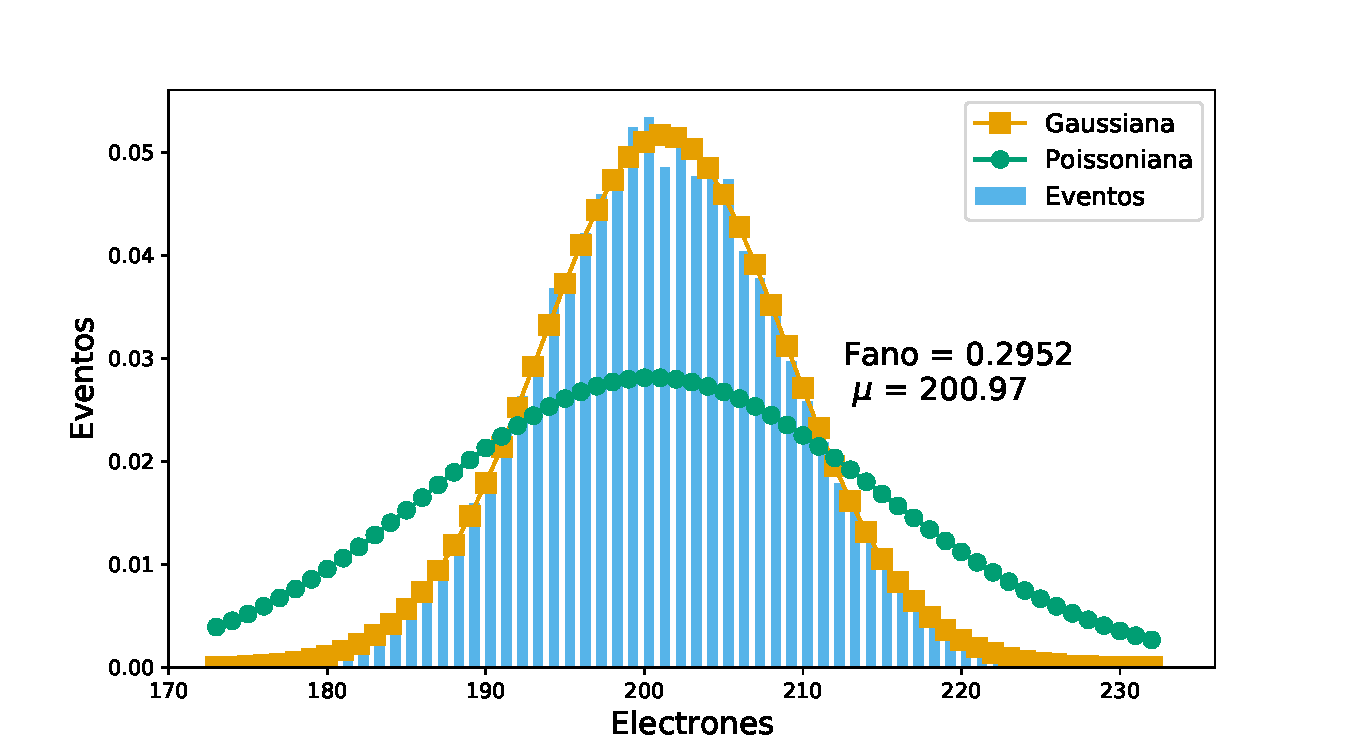
\includegraphics[scale=0.35]{Figs/Orden0_fano0.pdf}
    \caption{\footnotesize{Como reproducir esta imagen: Directorio (base) igna@Igna:~/Escritorio/Tesis2021/simulacion electrones\$ y correr ./SimuC2PyandPlot.py con parámetros: trials = 20000, distancia = 30000, atraviesa = 0 y branch git Master}}
    \label{fig:SimulacionOrden0Fano0}
\end{figure}

\begin{figure}[H]
%Para hacer este gráfico hay que correr el script que está en esta carpeta /home/igna/Escritorio/Tesis2021/Figs/Figuras_Apendice_Simulaciones/pys_para_plots y se llama Orden0_simu_SI_atraviesa.py con los datos de esta carpeta /home/igna/Escritorio/Tesis2021/Figs/Figuras_Apendice_Simulaciones/txts_para_plots y se llama orden0_simu_SI_atraviesa.txt
    \centering
    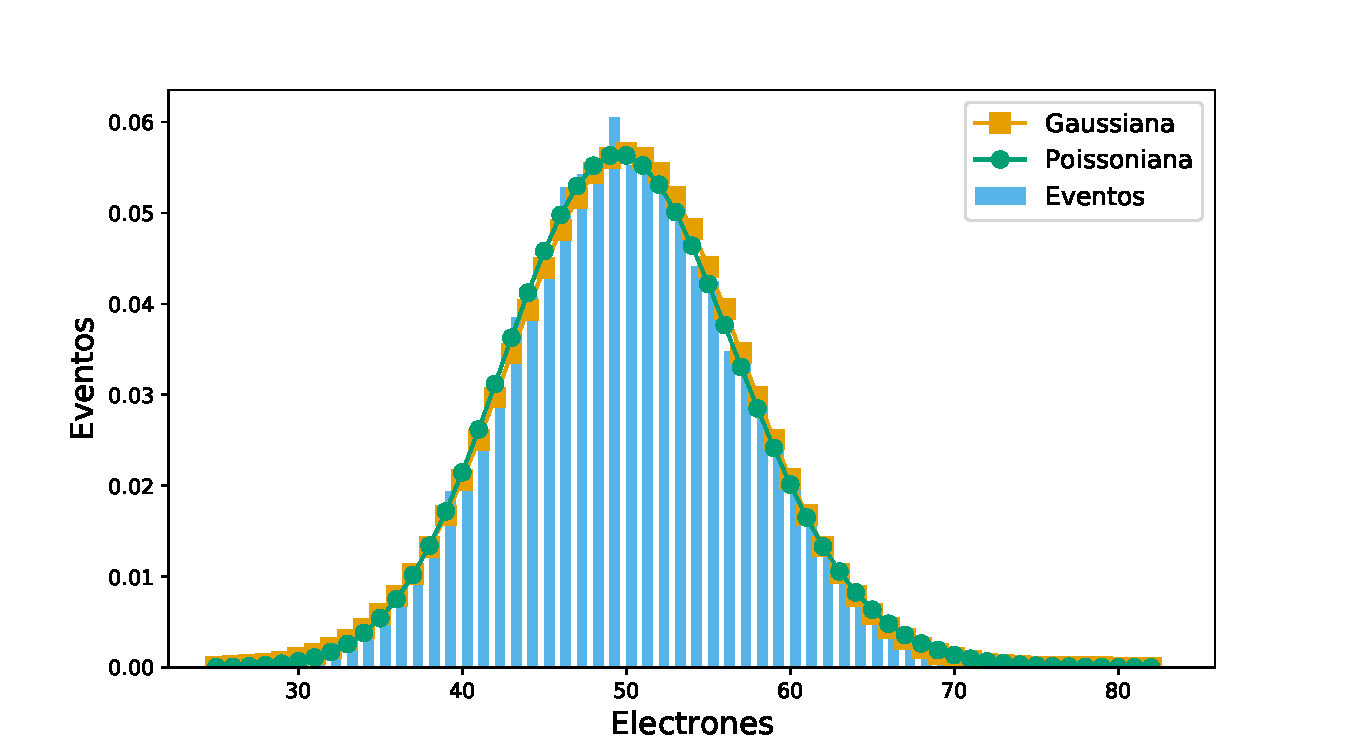
\includegraphics[scale=0.35]{Figs/Orden0_fano1.pdf}
    \caption{\footnotesize{Como reproducir esta imagen: Directorio (base) igna@Igna:~/Escritorio/Tesis2021/simulacion electrones\$ y correr ./SimuC2PyandPlot.py con parámetros: trials = 20000, distancia = 5000, atraviesa = 0 y branch git Master}}
    \label{fig:SimulacionOrden0Fano1}
\end{figure}
\noindent Si bien este modelo de juguete es una sobre-simplificación del proceso de dispersión real, los resultados de este están en concordancia con la hipótesis de que el factor de Fano es menor a $1$ debido a que la partícula incidente deposita toda su energía en el material.\\
\indent Con el fin de explorar mejor esta hipótesis, se propuso mejorar el modelo de la simulación Montecarlo. Esta vez considerando la posibilidad de que la partícula incidente pierda energía, además de por ionización, por emisión de fonones de la red. En este sentido se combinaron ideas de los trabajos de R.C. Alig et al.\cite{Alig} y K. Ramanathan \cite{Ramanathan}. En el primero proponen un modelo en el que la partícula incidente interactúa con el material, generando pares electrón-hueco por ionización en forma de cascada y, eventualmente, perdiendo energía por emisión de fonones. La forma en el que la partícula incidente va perdiendo energía depende fuertemente de la energía que tiene al momento de generar un par electrón-hueco. Esta dependencia está modelada en el segundo trabajo y lo llaman \textit{modelo simplificado}, donde proponen que la energía $E$ que se transfiere a para generar pares electrón-hueco se reparte según una distribución Beta, de la forma
\begin{equation*}
    p(x|\alpha) = \frac{2}{B(\alpha)} x^{\alpha - 1}(1-x)^{\alpha - 1}
\end{equation*}
donde $x = \frac{E}{E_{r} - E_{g}}$ es la variable aleatoria, con $E_{r}$ la energía inicial de la partícula en cada ionización, $E_{g}$ es la energía del gap del Silicio y $E$ es la fracción de energía va a parar a un nuevo par electrón hueco. Utilizando esta distribución para generar realizaciones de la variable aleatoria $x$, se puede despejar el valor de $E$ que es la energía transferida para generar pares electrón-hueco, para este modelo. Por otro lado, $B(\alpha)$ es la función Beta con un único parámetro $\alpha$, y viene dada, para el caso general por
\begin{equation*}
    B(\alpha, \beta) 
    = \frac{\Gamma(\alpha)\Gamma(\beta)}{\Gamma(\alpha) + \Gamma(\beta)}
\end{equation*}
y, para este caso particular, el parámetro $\beta = \alpha$ y $\alpha$ es el parámetro dependiente de la energía $E_{r}$ que determina el régimen de distribución de la energía, o en otras palabras, la forma de la distribución. \\
\indent La razón de la utilización de la distribución Beta para modelar como se reparte la energía en la generación de pares electrón-hueco por ionización:
\begin{itemize}
    \item \textbf{A bajas energías de la partícula incidente}, se tienen distribuciones muy picudas en los extremos posibles: $E = 0$ y $E = E_{R}+E_{g}$,
    \item \textbf{A energías mucho mayores que la energía del gap}, $E_{R} >> E_{g}$: Se tiene una distribución aproximadamente uniforme,
    \item \textbf{A energías entre $3.4\,eV$ - $4.2\,eV$ } se tiene una distribución de energía muy picuda en el medio de $x = E/(E_{R} - E_{g})$.
\end{itemize}
y estos tres casos pueden resumirse utilizando la Beta con el parámetro $\alpha$ adecuado. Para energías bajas, el parámetro $\alpha$ tiende a cero y se tiene una distribución con máximos en los extremos del intervalo. Para energías entre $3.4\,eV$ y $4.2\,eV$ se tiene una distribución con un máximo en el medio del intervalo y el parámetro $\alpha$ puede tender a infinito. Por último, para energías mucho mayores a la energía del gap, el parámetro $\alpha = 1$ y la distribución es uniforme. Estos casos se resumen el gráfico de la figura \ref{fig:BetaDist}.
\begin{figure}[H]
% Este gráfico se hace con el script que está acá: /home/igna/Escritorio/Tesis2021/Figs/Figuras_Apendice_Simulaciones/pys_para_plots DistBetaFig.py
    \centering
    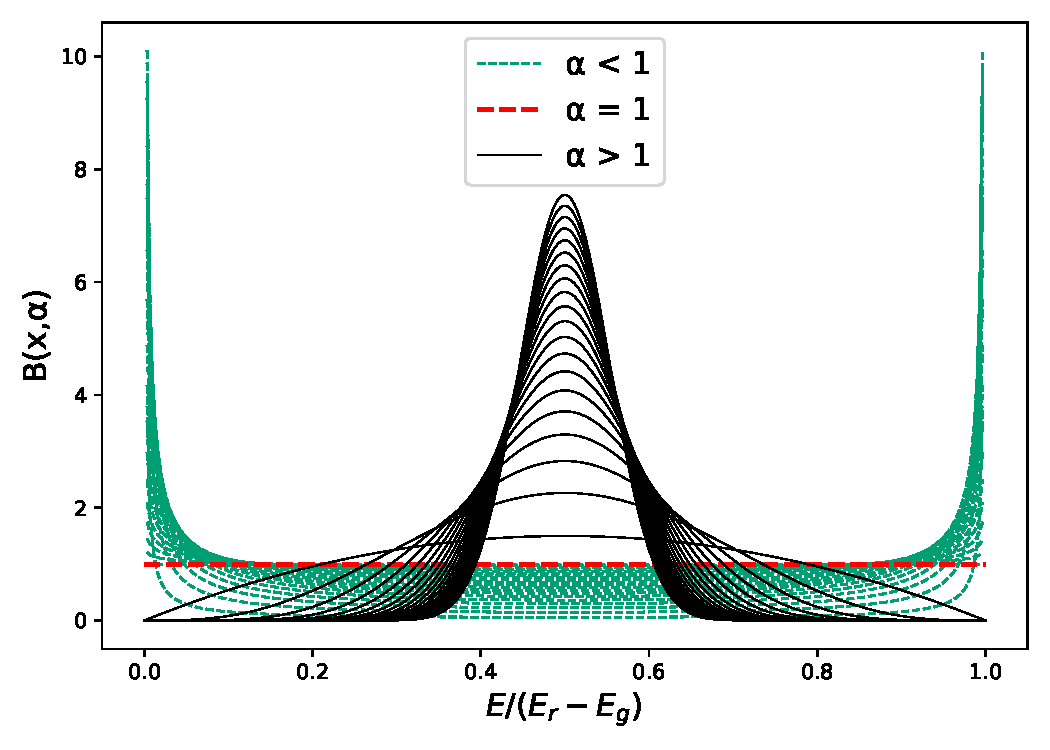
\includegraphics[scale=.7]{Figs/BetaDistFig.pdf}
    \caption{\footnotesize{Distribución Beta para diferentes valores del parámetro $\alpha$}}
    \label{fig:BetaDist}
\end{figure}

\subsection{Orden uno}
\noindent Utilizando ideas tomadas de los trabajos anteriormente citados, se realizaron simulaciones Montecarlo para intentar reproducir el mecanismo de creación de pares electrón-hueco por ionización. Para este caso se tuvo en cuenta la posibilidad de disipación de energía por emisión de fonones, a una energía fija de $\hbar\omega_{0} = 0.063\,eV$.\\
\indent El mecanismo de cascada por el cual se producen las ionizaciones consiste en que para una dada energía inicial $E_{R}$, una fracción de esa energía se utiliza para generar un par electrón-hueco y la energía restante vuelve a fraccionarse para generar otros pares electrón-hueco. Estos pares generados, a su vez, utilizan fracciones de esa energía que les fue entregada para generar otros pares, en un proceso que se repite hasta que la energía disponible para repartir en cada rama de la cascada es menor a la energía del gap del Silicio y no es suficiente para generar más pares. Durante todo este proceso existe una probabilidad no nula de que parte de la energía se pierda por emisión fonones en la red.\\
\indent Se define una probabilidad $P_{eh}$ para la cual se produce ionización y una probabilidad $1 - P_{eh}$ para la cual se produce emisión de fonones. Esta probabilidad depende de la energía inicial, al igual que el parámetro $\alpha$ de la distribución Beta, y viene dada por
\begin{equation}
    P_{eh}(E_{R}) = 
    \left[
        1 + \frac{\Gamma_{ph}(E_{R})}{\Gamma_{eh}(E_{R})}
    \right]^{-1}
        \label{ec:ProbabilidadIonizacion}
\end{equation}
donde 
\begin{equation*}
    \frac{\Gamma_{ph}(E_{R})}{\Gamma_{eh}(E_{R})}
    = A\frac{105}{2\pi}\frac{(E_{R} - \hbar \omega_{0})^{1/2}}{(E_{R} - E_{g})^{7/2}}
\end{equation*}
con $A = 5.2\,eV^{3}$, que es una constante fenomenológica que contiene información microscópica del sistema y que además puede ajustarse para reproducir valores medidos experimentalmente. Por otro lado, $\Gamma_{ph}$ y $\Gamma_{eh}$ son las tasas de producción de fonones y pares electrón-hueco, respectivamente.\\
\indent El resultado de la simulación es simplemente el número de pares ionizados a partir de la energía inicial $E_{R}$. De esta puede verse la distribución de la cantidad de pares generados y además calcular tanto su varianza como su esperanza, para así obtener el factor de Fano.\\
\indent Otro factor a tener en cuenta en la simulación es la conservación de la energía durante el proceso de creación de pares. Puede considerarse que la energía transferida al ionizar, puede utilizarse totalmente para ionizar otros pares, o puede considerarse que siempre que se de una ionización, habrá una pequeña parte de energía que se pierde y no puede ser utilizada, es decir, que no se conserva la energía.\\
\indent Por último, en este tipo de simulación solo se puede considerar el caso en el que la partícula disipa toda su energía en el interior del material, de modo que se esperan valores para el factor de Fano menores a la unidad.

\subsubsection{Implementación}
\noindent La implementación de los códigos que ejecutan la simulación Montecarlo se realizó con los lenguajes C y Python. Con C se realiza todo el trabajo de alto costo computacional, mientras que Python cumple un rol de interfaz para los parámetros de la simulación, como ser, por ejemplo, la energía inicial, la cantidad de corridas del Montecarlo, etc.\\
\indent A grandes rasgos, en el código en C están implementadas las funciones que hacen los cálculos antes mencionados: El cálculo de la probabilidad de ionización $P_{eh}$ a partir de la expresión \eqref{ec:ProbabilidadIonizacion}, el cálculo del parámetro $\alpha = \alpha(E_{R})$ según la energía $E_{R}$ para la distribución Beta, a partir de la cual se genera una realización de la variable aleatoria de la que se puede despejar la energía transferida a un par electrón-hueco por ionización. Finalmente, por recursión se simulan los procesos de ionización en cascada y se cuenta la cantidad final de electrones ionizados.\\
\indent Por otro lado, la función del código en Python no es más ejecutar el programa en C las veces que sean necesarias y con los parámetros iniciales de interés para obtener el resultado buscado.\\
\indent Más en detalle, el programa en C consta de un total de $6$ funciones, las cuales se listan a continuación con una breve descripción de su funcionamiento
\begin{enumerate}[label=\arabic*., listparindent=1.5em]
    \item \verb|Random()|: Es simplemente una función que genera realizaciones \verb|p_rand| de una distribución uniforme, entre $0$ y $1$. Se usa para generar una probabilidad de comparación en el Montecarlo.
    \item \verb|Peh(E_r, A)|: Es la función encargada de realizar el cómputo de la probabilidad de ionización, según la ecuación \eqref{ec:ProbabilidadIonizacion}, a partir de la energía $E_{R}$, que es un parámetro inicial que es ingresado con Python. Esta probabilidad \verb|p_eh| se compara con \verb|p_rand| en el algoritmo de aceptación del Montecarlo.
    \item \verb|alpha(E_r)|: Calcula el valor del parámetro $\alpha$ en base al valor del parámetro \verb|E_r|. Si bien el parámetro \verb|E_r| es un parámetro inicial, que para el Flúor es $677\,\si{eV}$, a medida que evoluciona el sistema, la energía se va perdiendo en ionizaciones y este parámetro es actualizado. Con cada actualización se calcula nuevamente el valor de $\alpha$ de para la distribución Beta. El valor del parámetro se calcula entonces como
    \begin{equation*}
        \alpha =
        \left\{
            \begin{matrix}
                0.1\ \mbox{si}\ E_{r} < E_{g}\\
                1\ \mbox{si}\ E_{g} < E_{r} < 2E_{g}\\
                1\ \mbox{si}\ 3.4\,\si{eV} < E_{r} < 4.2\,\si{eV}\\
                0.0207E_{r} + 0.95435\ \mbox{en otro caso.}
            \end{matrix}
        \right.
    \end{equation*}
    \item \verb|evolucionar(E_r, A, E_loss, rand_beta)|: Genera la evolución del sistema mediante Montecarlo, haciendo uso de las funciones anteriores. Implementa un bucle \verb|while|, cuya condición es que se repita el proceso mientras que la energía \verb|E_r| sea mayor que la energía del gap del Silicio \verb|E_g|. Dentro del bucle se calcula la probabilidad \verb|p_eh| de ionización, el parámetro $\alpha$, que luego es usado para generar un número pseudo aleatorio con distribución Beta del cual despejar la fracción de energía \verb|E_traf| que va a un par electrón hueco al ionizar y, por último, genera el número pseudo aleatorio de distribución uniforme con cual comparar la probabilidad de ionización en el Montecarlo.\\
    \indent Una vez que se tienen estos valores, siempre y cuando se cumpla que la probabilidad de ionizacion \verb|p_eh| sea mayor que \verb|p_rand| y que al mismo tiempo la fracción de energía \verb|E_tranf| sea mayor que $3.75\,\si{eV}$\footnote{Condición que cobra gran relevancia en los resultados y se explica en más datella en la siguiente sección} (valor medio para la energía de creación electrón hueco $\varepsilon_{\eh}$), entonces se actualiza el valor de la energía inicial \verb|E_r| restándole la fracción de energía transferida. Además, también, se guardan en una lista la resta entre las energías transferidas \verb|E_r| y la energía perdida por ionización \verb|E_loss|. Esta última es un parámetro configurable de la simulación, en la cual se puede considerar el caso donde la energía se conserva y \verb|E_loss = 0| o el caso en el que no hay conservación de energía y \verb|E_loss|$\neq$\verb|0|. Notar que la cantidad de elementos de la lista será la cantidad de pares electrón-hueco generados por una rama de la cascada con energía inicial \verb|E_r|. Luego, cada elemento de la lista se transforma, para otra rama, en \verb|E_r|, generando una nueva lista. Repitiendo con todas las energías de toda la lista y todas las sublistas, se pueden contar los electrones ionizados.\\
    \indent De no cumplirse la condición del Montecarlo, el sistema pierde energía por emisión de fonones, es decir, la energía \verb|E_r| se actualiza restándole un valor fijo de energía $\hbar \omega = 0.063\,\si{eV}$. El resultado de esta función es una lista con las energías de una sola rama de la cascada.
    \item \verb|recursion(E_r, A, E_loss, rand_beta)|: Esta función cuenta de manera recursiva la cantidad de electrones ionizados durante la cascada. La recursion, en este caso, tiene la ventaja de que es muy sencilla de implementar, pero tiene como desventaja que no es tan sencillo entender por qué funciona correctamente.\\
    \indent Lo primero que hace esta función es generar una lista energías, \verb|Energia|, llamando a la función \verb|evolucionar()| y luego se itera sobre todas estas, contando la cantidad total de elementos que posee. Esas energías son las que fueron usadas para ionizar un par electrón hueco, así que la cantidad de energías que alberga la lista es equivalente a la cantidad de pares generados. Notar que a \verb|recursion()| se le pasa como argumento \verb|E_r|. De modo que si dentro de \verb|recursion()| se vuelve a llamar a ella misma, pero ahora en vez de usar como argumento \verb|E_r|, se usa el primer elemento de la lista \verb|Energia|, es decir \verb|Energia[0]|, se produce una nueva lista a partir de una energía inicial menor y contando la cantidad de elementos. Si ahora se repite para el elemento \verb|Energia[1]|, se genera otra lista de energías. El proceso se repite hasta que todas las energías de la lista original se agotaron. Luego, las sublistas generadas repiten el proceso para todos sus elementos hasta que eventualmente la energía de las listas no es suficiente para seguir ionizando y el proceso termina.\\
    \indent El valor de salida de la función \verb|recursion()| es un entero y contabiliza la cantidad de elementos encontrados en la lista, es decir, la cantidad de electrones ionizados. Durante el proceso de recursión se van sumando todas las cantidades de carga ionizada en cada paso y finalmente se obtiene la carga total generada durante la cascada.
    \item \verb|main()|: Esta se encarga de llevar adelante las repeticiones del experimento con el fin de obtener estadística. Además, en esta se definen los parámetros necesario para la simulación, como ser la energía inicial \verb|E_r|, el parámetro \verb|A|, el valor de la energía que se pierde por ionizar \verb|E_loss|, la cantidad de experimentos que se quieren realizar \verb|trials| y la generación de un archivo \verb|.txt| con los datos obtenidos para ser levantados posteriormente con Python.
\end{enumerate}
Cabe destacar que de esta simulación el único resultado que se obtiene es la distribución de carga para una dada energía inicial $E_{r}$. Es decir, no puede conocerse ningún proceso intermedio o la \textit{historia} del proceso, solo la cantidad total de electrones generados.

\subsubsection{Simulaciones}
\noindent Se realizaron las simulaciones partiendo de una energía inicial $E_{r} = 677\,\si{eV}$, correspondiente a los rayos $X$ de Flúor, que es el principal objeto de estudio de este trabajo. Los valores de los parámetros fueron extraídos de la bibliografía y son $A = 5.2\,\si{eV}^{3}$, la energía del gap $E_{g} = 1.1\,\si{eV}$, la energía de creación electrón-hueco promedio $\varepsilon_{eh} = 3.75\,\si{eV}$ y la energía perdida cada vez que se emiten fonones $\hbar \omega = 0.063\,\si{eV}$. El resto de los parámetros son configurables y se variaron para ver los diferentes resultados de la simulación, como ser la pérdida de energía al ionizar $E_{loss}$ y la cantidad de repeticiones del experimento \textit{trials}. La simulaciones se efectuaron con no menos de $5000$ repeticiones y con diferentes valores de $E_{loss}$.\\
\indent Se simuló el proceso de cascada con con diferente cantidad de \textit{trials}, es decir, de repeticiones del experimento, partiendo desde $5000$ hasta incluso $100000$ para asegurar la robustez de la estadística. Además, con el fin de poder caracterizar mejor las dependencias entre parámetros en la simulación, se hizo un barrido sobre la pérdida de energía $E_{loss}$ para conocer la dependencia de los resultados respecto de este, partiendo desde $0\,\si{eV}$ de pérdida de energía hasta $7\,\si{eV}$ de pérdida de energía por cada ionización (equivale a perder casi $4$ veces la energía del gap del Silicio).\\
\indent Con estos barridos se vio la dependencia de tanto del factor de Fano, como de la energía de creación electrón-hueco y del valor medio de carga ionizada al variar el valor de la energía que se pierde con cada ionización. Se observó que estos parámetros son muy sensibles a la pérdida de energía del sistema, obteniéndose resultados con cambios de regímenes muy pronunciados, particularmente, cuando la energía perdida por ionización coincide con el valor $E_{loss} = 3.75\,\si{eV}$, que casualmente es la energía de creación electrón-hueco promedio y que se usó en la simulación como un parámetro fijo en la función \verb|evolucionar()|.

\subsubsection{Resultados}
\noindent Los resultados de las simulaciones del factor de Fano se ven en los gráficos de las figuras \ref{fig:Simulacion1rden1Fano1} y \ref{fig:Simulacion1rden1Fano2}. Ambos muestran la distribución de carga simulada, un ajuste Gaussiano a ese histograma, usando el $\mu$ y el $\sigma$ generado a partir de los datos y a su vez la forma de la Poissoniana que corresponde a ese valor medio $\mu$. Se ve claramente como la distribución de carga está lejos de parecerse a una distribución de Poisson y por ello el factor de Fano se aleja de la unidad.\\
\indent El primer caso corresponde a una simulación en la que se repitió el mismo experimento de cascada $100000$ veces para tener una buena robustez estadística, mientras que en el segundo caso se usaron $10000$ repeticiones del experimento. En la figura \ref{fig:FanoConvergencia} se observa la convergencia de los valores del factor de Fano a medida que aumenta el número de experimentos.
\begin{figure}[h]
%Este gráfico se puede hacer con el script GrafFanoConvergencia.py que esta en este directorio /home/igna/Escritorio/Tesis2021/Figs/Figuras_Apendice_Simulaciones/pys_para_plots
    \centering
    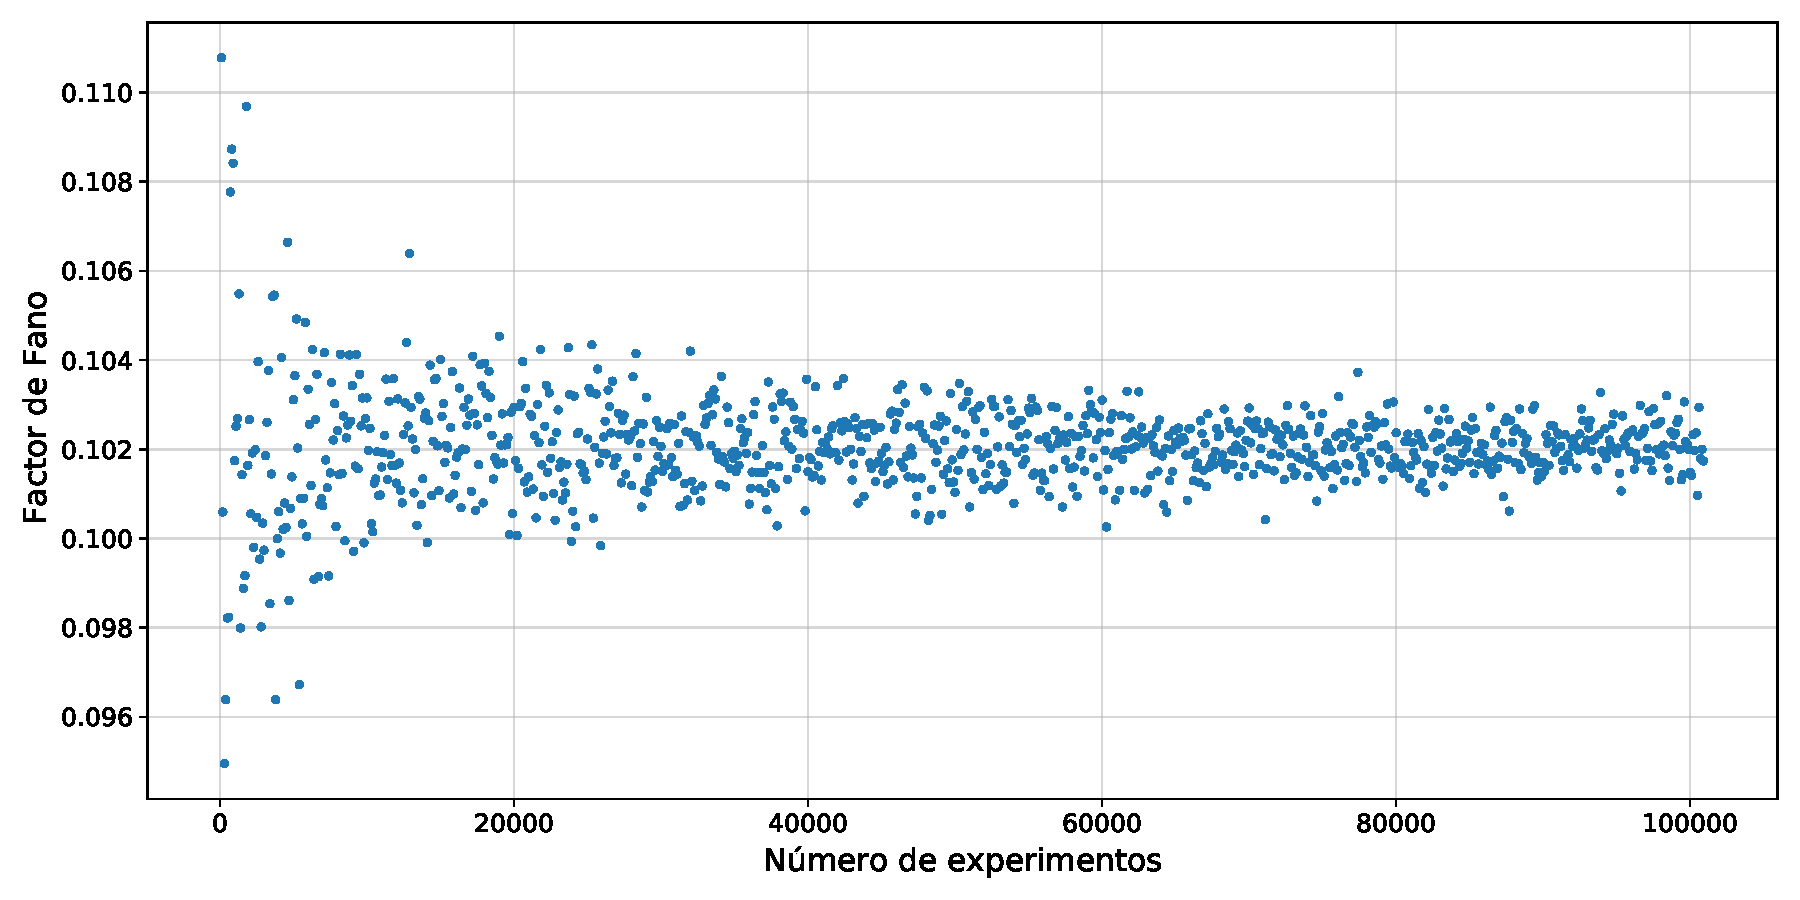
\includegraphics[scale=0.5]{Figs/FanoConvergencia.pdf}
    \caption{\footnotesize{Dispersión de los valores del Factor de Fano cada cantidad de repeticiones del experimento, partiendo desde $100$ repeticiones hasta 100900 repeticiones.}}
    \label{fig:FanoConvergencia}
\end{figure}
Para $10000$ repeticiones se ve que los valores del factor de Fano están acotados entre $\sim 0.106$ y $\sim 0.098$, mientras que para $100000$ repeticiones están acotados entre $\sim 0.104$ y $\sim 0.100$. Se nota claramente la mejora en la estadística.\\
\indent En la figura \ref{fig:Simulacion1rden1Fano1} se puede ver lo bien que se ajusta una distribución Gaussiana al histograma. En este caso el factor de Fano correspone a $F = 0.1021$ y el valor medio de carga $\mu = 192$, un valor bastante corrido a la derecha respecto del valor esperado, cercano a $\mu = 181$.
\begin{figure}[h]
%Los datos para este gráfico están en /home/igna/Escritorio/Tesis2021/Figs/Figuras_Apendice_Simulaciones/txts_para_plots Distribucion_carga_simulada_100k.txt Para modificar el graf hay que correr el .py que están en /home/igna/Escritorio/Tesis2021/Figs/Figuras_Apendice_Simulaciones/pys_para_plots Fano_100k_dist_carga.py
    \centering
    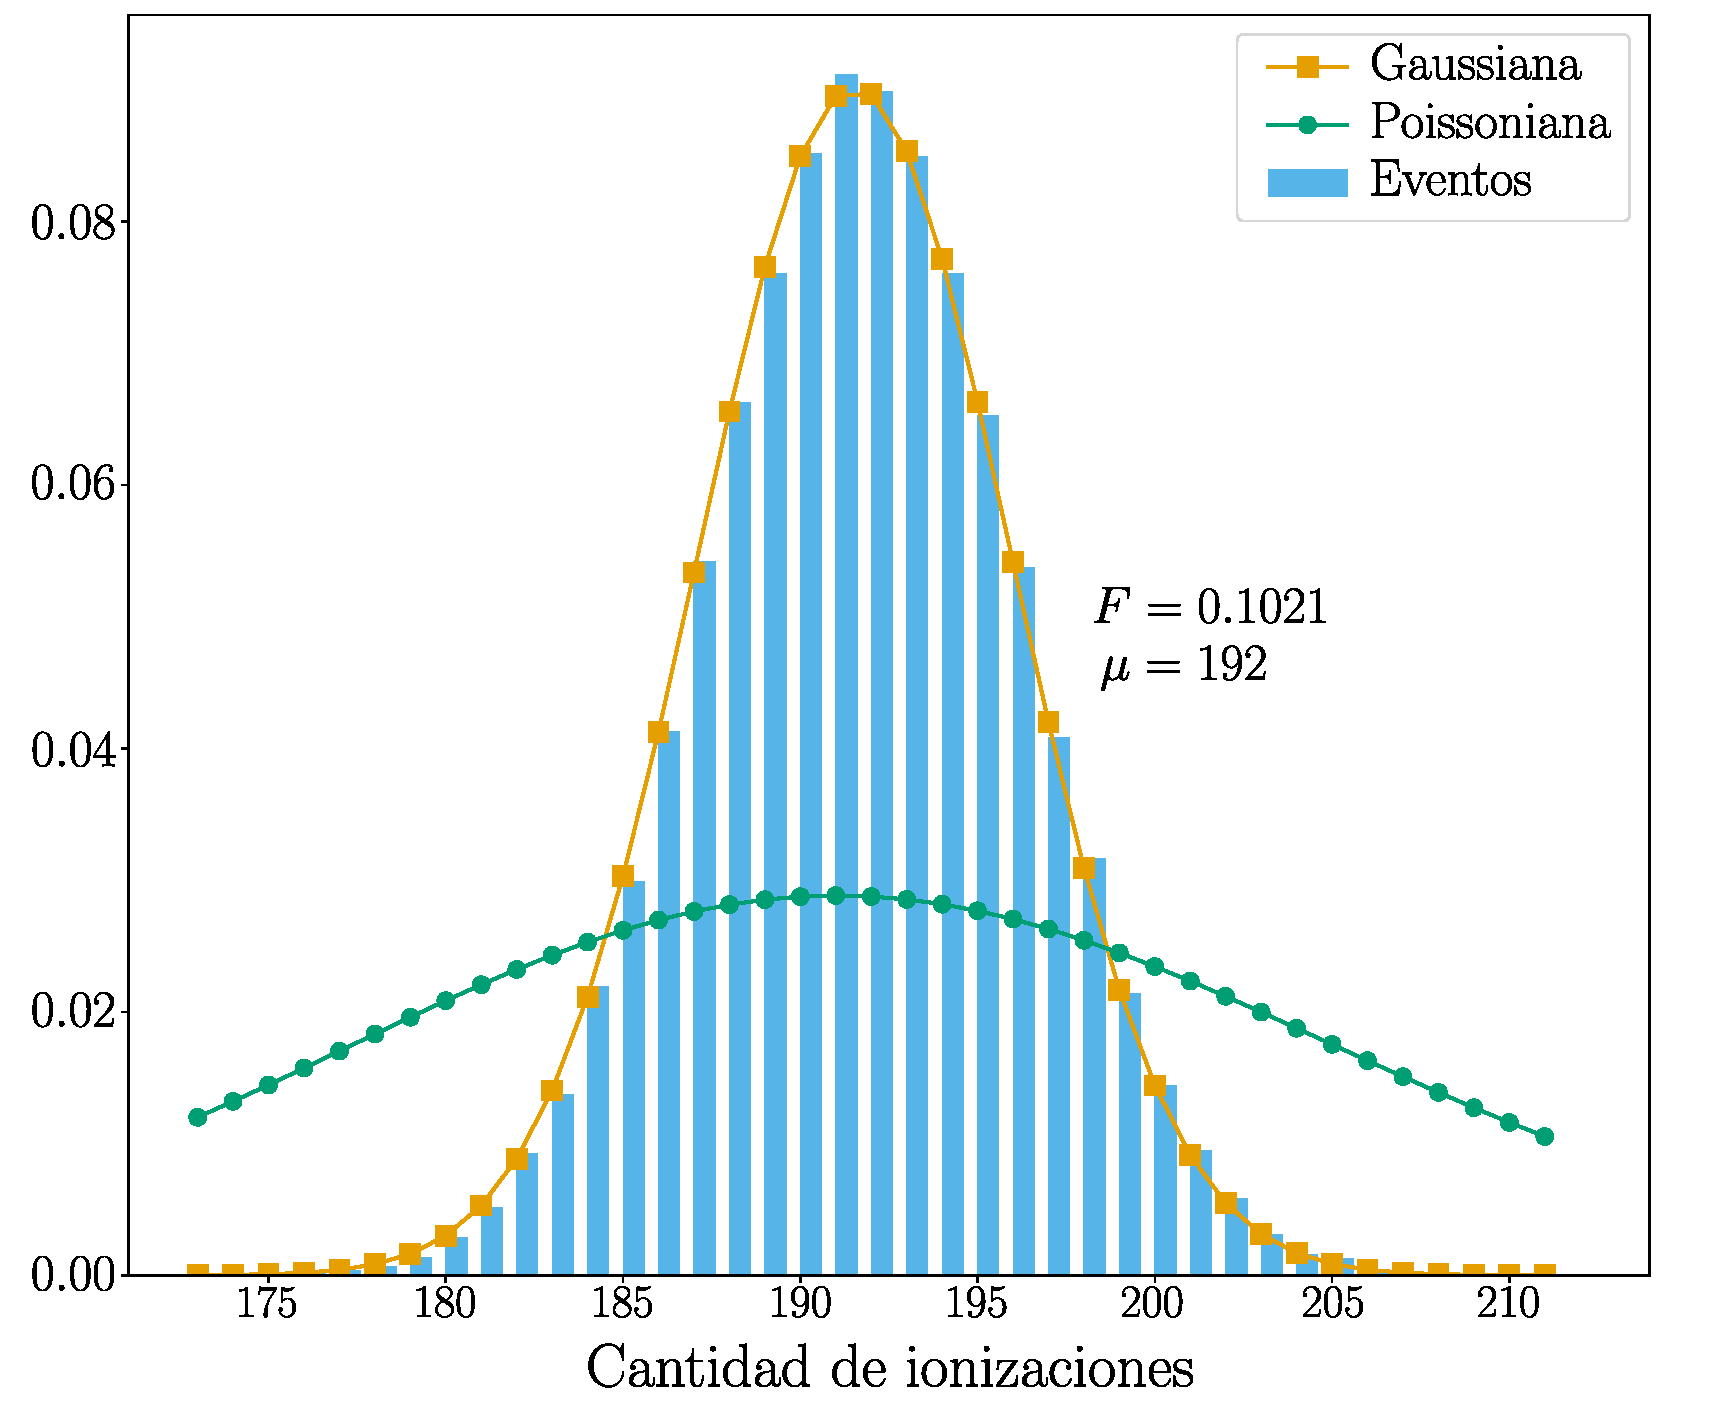
\includegraphics[scale=0.35]{Figs/Fano_677_Eloss0_100ktrials.pdf}
    \caption{\footnotesize{Distribución de carga simulada con el método de Montecarlo, con parámetro $A = 5.2\,\si{eV}^{3}$ y $100000$ \textit{trials} para obtener la mejor estadística posible. Se observa un valor medio $\mu = 192$, lo cual representa un corrimiento hacia la derecha del valor esperado para el pico de los rayos $X$ del Flúor, que es al rededor de $181$ electrones.}}
    \label{fig:Simulacion1rden1Fano1}
\end{figure}
\noindent Para el segundo caso, en la figura \ref{fig:Simulacion1rden1Fano2}, se modificó el valor del parámetro $A$ de forma que el pico coincida con lo esperado, que son $\mu = 181$ electrones. El valor de $A$ que cumple esa condición es $A = 20\,\si{eV}^{3}$, valor $5$ veces mayor al propuesto en la bibliografía para describir macroscópicamente las propiedades del Silicio.
\begin{figure}[h]
%Los datos para este gráfico están en /home/igna/Escritorio/Tesis2021/Figs/Figuras_Apendice_Simulaciones/txts_para_plots Distribucion_carga_simulada_10k.txt Para modificar el graf hay que correr el .py que están en /home/igna/Escritorio/Tesis2021/Figs/Figuras_Apendice_Simulaciones/pys_para_plots Fano_10k_dist_carga.py
    \centering
    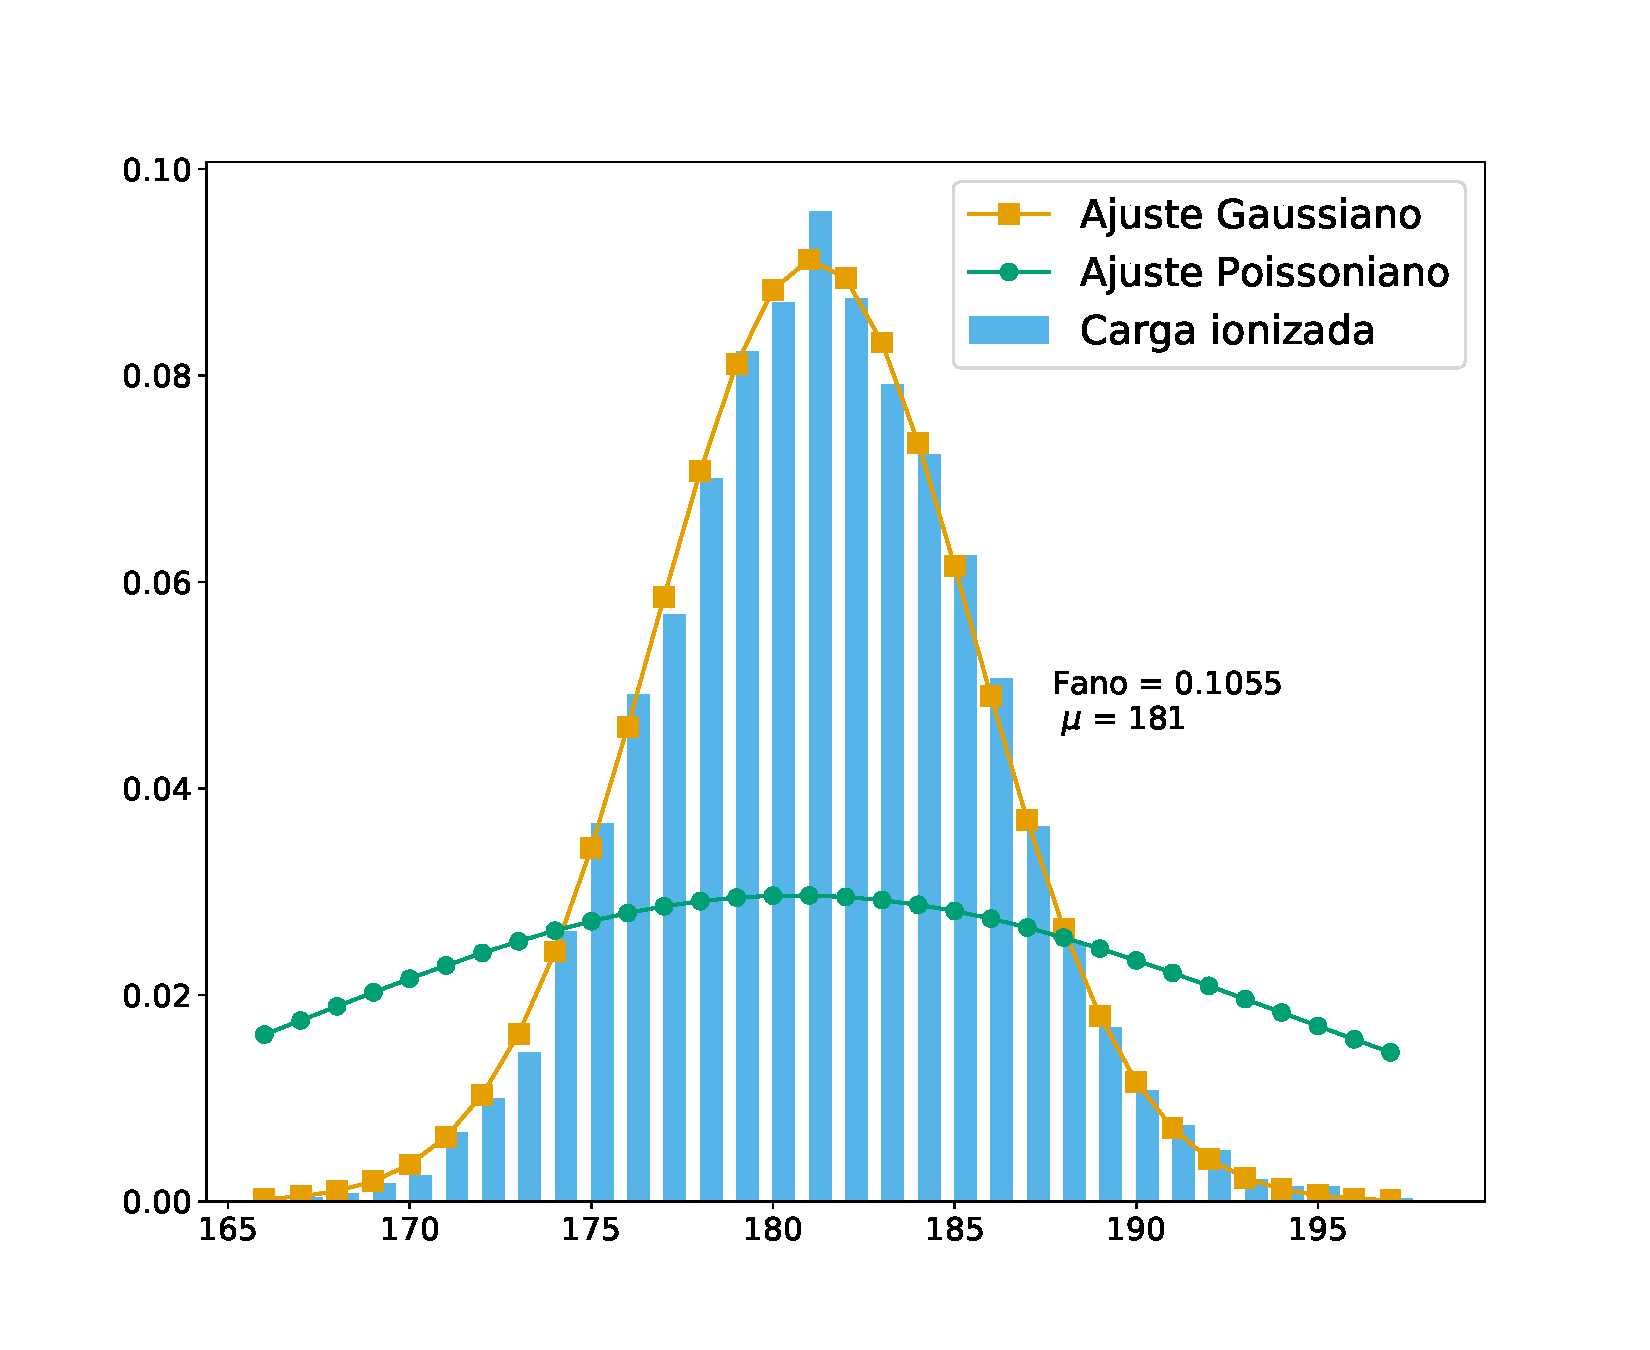
\includegraphics[scale=0.35]{Figs/Fano_677_Eloss0_10ktrials.pdf}
    \caption{\footnotesize{Distribución de carga simulada con el método de Montecarlo, forzando el parámetro $A$ para que el pico se encuentre en los $181$ electrones esperados para los $677\,\si{eV}$ de energía de los rayos X del Flúor. En este caso $A=20$ y se usaron solamente $10000$ \textit{trials}.}}
    \label{fig:Simulacion1rden1Fano2}
\end{figure}
El factor de Fano en este caso es de $F = 0.1055$, que está contenido entre las bandas esperadas para la cantidad de estadística utilizada en esta simulación. La razón por la cual usar menor estadística en este caso fue porque no era necesaria tanta robustez.\\
\indent En ambos casos el valor del factor de Fano es muy semejante y da, como se esperaba, alrededor de un orden de magnitud inferior a la unidad. Los valores esperados son << buscar valores esperados >>.\\
\indent En cuanto a los barridos, la dependencia del factor de Fano con la energía $E_{loss}$ (y al igual que la energía de creación electrón-hueco y el valor medio de carga ionizada) presenta un cambio de régimen abrupto cuando se cruza el umbral $E_{loss} = 3.75\,\si{eV}$. En la figura \ref{fig:FanoVsEloss} puede verse claramente este cambio de régimen. También se observa que cuando hay conservación de la energía, es decir, $E_{loss} = 0$, es cuando se obtiene un factor de Fano más semejante al observado experimentalmente, que está cerca de $0.1$.
\begin{figure}[h]
%a) Esta figura se puede hacer con los datos de: fano_Eloss_mu_vec.txt que está en el directorio /home/igna/Escritorio/Tesis2021/Figs/Figuras_Apendice_Simulaciones/txts_para_plots usando el .py Barridos_mu_Eloss_fano.py que está en /home/igna/Escritorio/Tesis2021/Figs/Figuras_Apendice_Simulaciones/pys_para_plots
    \centering
    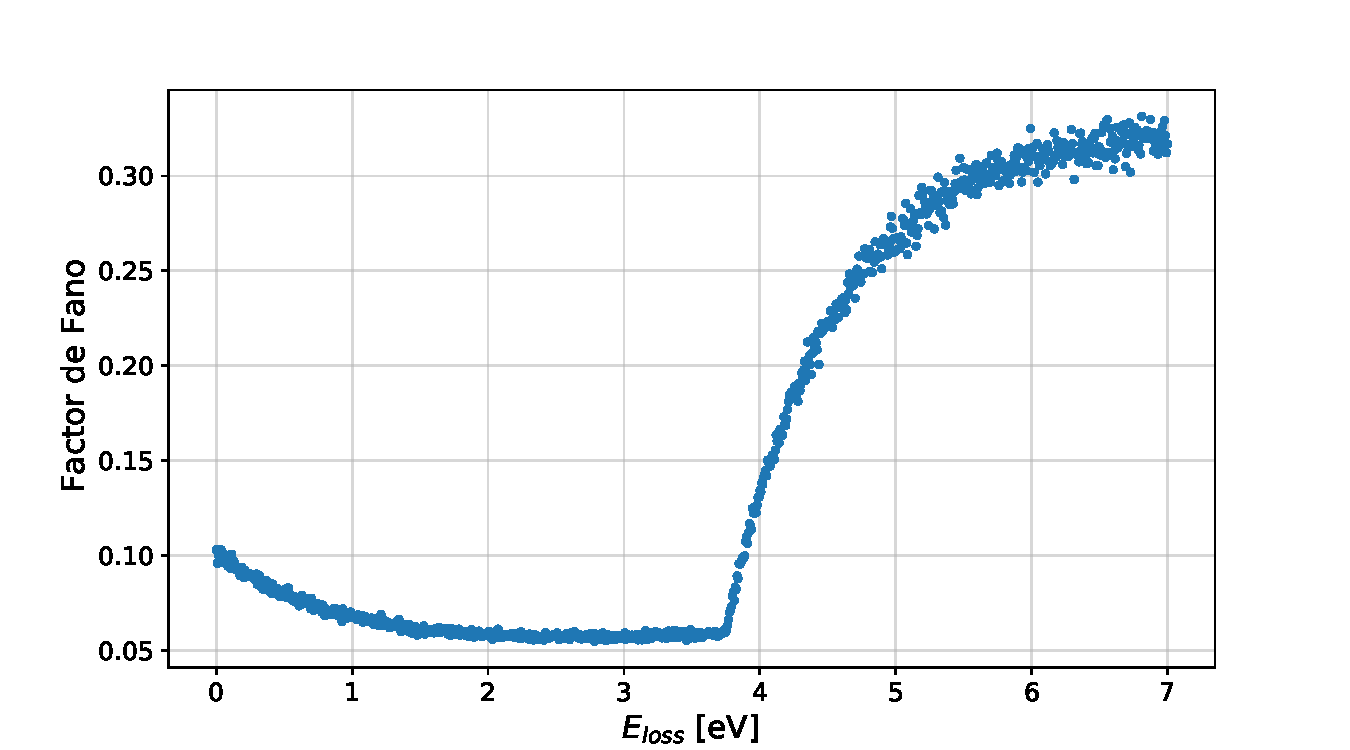
\includegraphics[scale=0.35]{Figs/Fano_vs_Eloss_5ktrials_0-7Eloss.pdf}
    \caption{\footnotesize{asd.}}
    \label{fig:FanoVsEloss}
\end{figure}
A medida que aumenta la pérdida de energía, el factor de Fano comienza a decrecer hasta que se alcanza los $3.75\,\si{eV}$ de pérdida de energía, donde se observa el cambio brusco en la curva, y se observa un aumento pronunciado de la misma, muy semejante a un punto crítico.\\
\indent De la misma forma, el valor media de la carga ionizada $\mu$ tiene un cambio de concavidad en la curva a medida que aumenta la cantidad de energía perdida por cada ionización, como se ve en la figura \ref{fig:ElossVsMu}

\begin{figure}[h]
% b) Esta figura se puede hacer con los datos de: fano_Eloss_mu_vec.txt que está en el directorio /home/igna/Escritorio/Tesis2021/Figs/Figuras_Apendice_Simulaciones/txts_para_plots usando el .py Barridos_mu_Eloss_fano.py que está en /home/igna/Escritorio/Tesis2021/Figs/Figuras_Apendice_Simulaciones/pys_para_plots
    \centering
    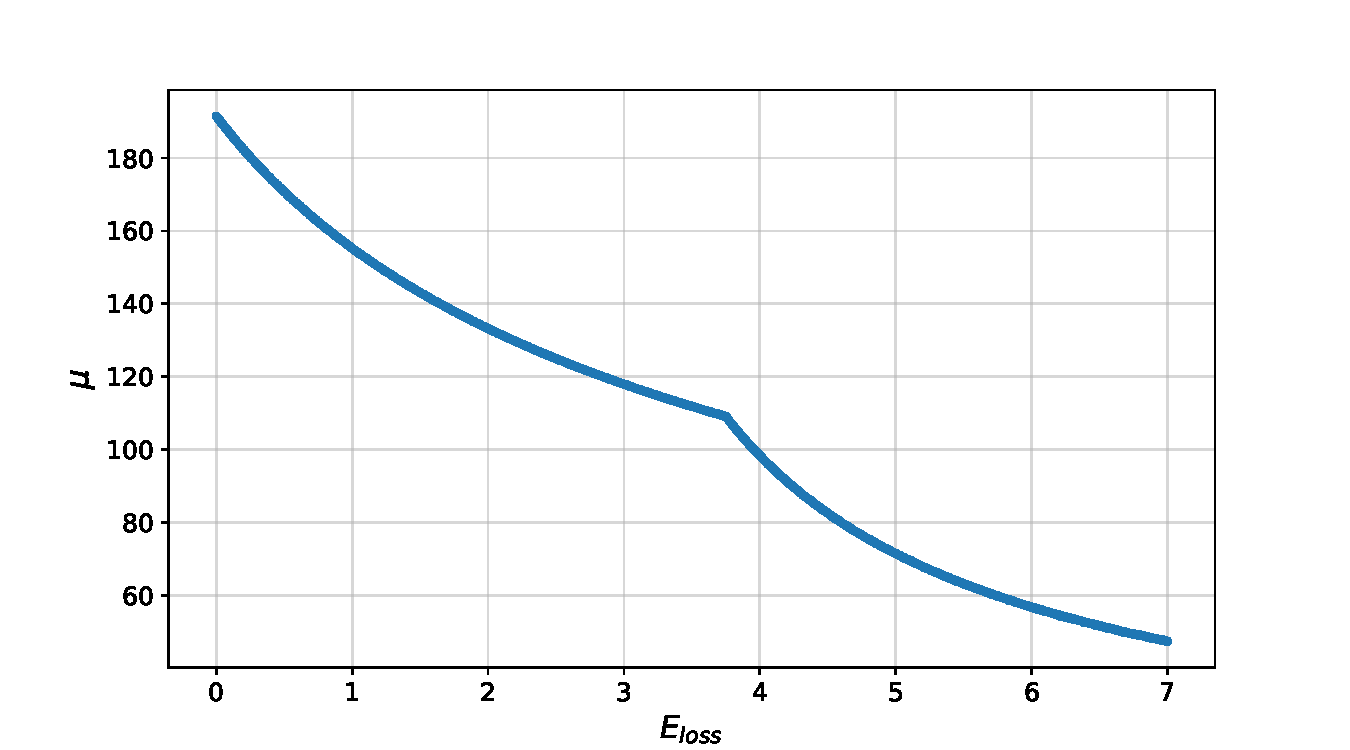
\includegraphics[scale=0.35]{Figs/ELoss_vs_mu_5ktrials_0-7Eloss.pdf}
    \caption{\footnotesize{asd.}}
    \label{fig:ElossVsMu}
\end{figure}
Nuevamente, los valores más cercanos a los medidos experimentalmente son los que corresponden a los casos en los que hay conservación de la energía.\\
\indent Por último, para la energía de creación electrón hueco, calculada a partir del valor medio de carga ionizada y la energía inicial $E_{R} = 677\,\si{eV}$, usando $\left\langle\varepsilon_{\eh} \right\rangle= 677\,\si{eV}/\mu$, claramente tendrá el mismo cambio de régimen en $3.75\,\si{eV}$, como se ve en la figura \ref{fig:CreacionHuecoVsEloss}
\begin{figure}[h]
%a) Esta figura se puede hacer con los datos de: fano_Eloss_mu_vec.txt que está en el directorio /home/igna/Escritorio/Tesis2021/Figs/Figuras_Apendice_Simulaciones/txts_para_plots usando el .py Barridos_mu_Eloss_fano.py que está en /home/igna/Escritorio/Tesis2021/Figs/Figuras_Apendice_Simulaciones/pys_para_plots
    \centering
    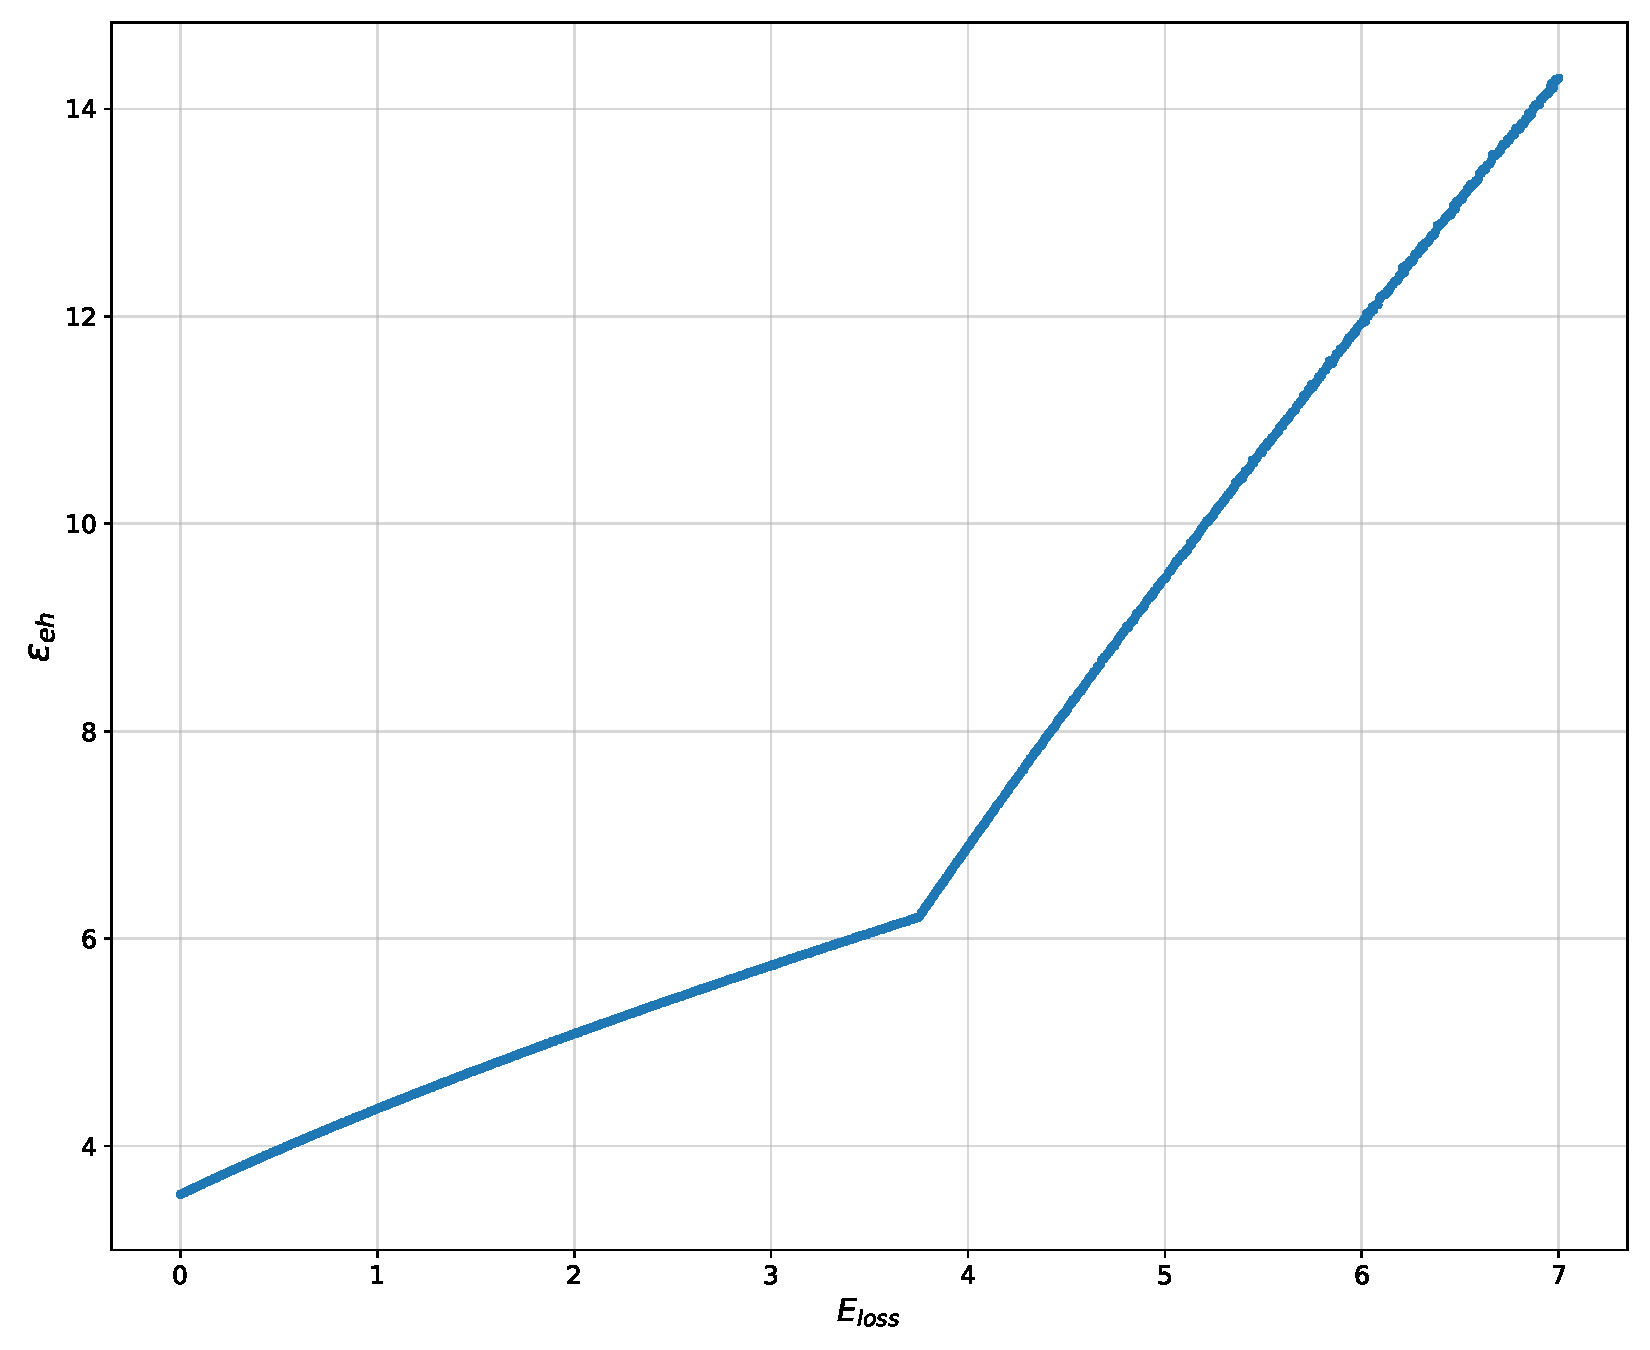
\includegraphics[scale=0.35]{Figs/E_eh_vs_Eloss_5ktrials_0-7Eloss.pdf}
    \caption{\footnotesize{asd.}}
    \label{fig:CreacionHuecoVsEloss}
\end{figure}
Con lo cual se observa que este Montecarlo \textit{de juguete} es muy sensible a dos parámetros muy importantes de la física real del sistema: La energía de creación electrón hueco, porque es el parámetro de la condición de \verb|evolucionar()| que determina si hay o no ionización; y la conservación de la energía. Se observa que cuando la energía se conserva en la simulación, se obtienen los resultados más cercanos a los observados experimentalmente y reportados en la bibliografía.